\documentclass[tikz,border=10pt]{standalone}
\begin{document}
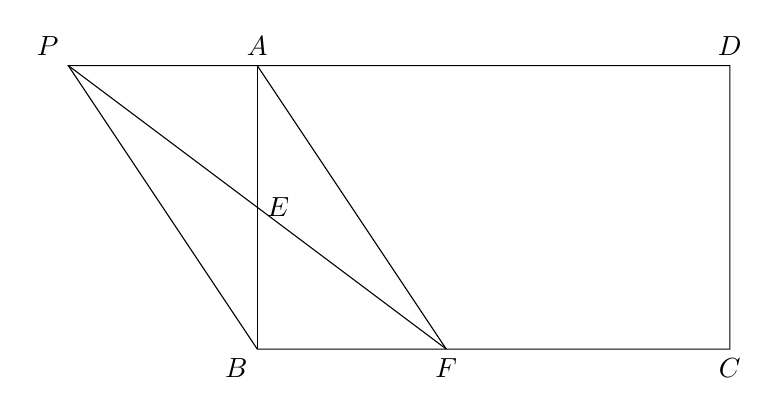
\begin{tikzpicture}[scale=1.2]
  \coordinate (P) at (0,3);
  \coordinate (A) at (2,3);
  \coordinate (D) at (7,3);
  \coordinate (B) at (2,0);
  \coordinate (F) at (4,0);
  \coordinate (C) at (7,0);
  \coordinate (E) at (intersection of P--F and A--B);
  \draw (P) -- (D) -- (C) -- (B) -- cycle;
  \draw (A) -- (B);
  \draw (P) -- (F);
  \draw (A) -- (F);
  \node[above left] at (P) {$P$};
  \node[above] at (A) {$A$};
  \node[above] at (D) {$D$};
  \node[below left] at (B) {$B$};
  \node[below] at (F) {$F$};
  \node[below] at (C) {$C$};
  \node[right] at (E) {$E$};
\end{tikzpicture}
\end{document}
